\title{Report on <CONFIG_CASE>  experiment}
\author{
        Jean-Marc Molines, ... \\
        MEOM- IGE - CNRS \\
        IGE-DRA-\todayiso
}
\date{\today}

\documentclass[12pt]{article}

\usepackage{graphicx}
\usepackage{url}
\usepackage{float}
\usepackage[french,english]{babel}
\usepackage{verbatim}
\usepackage[T1]{fontenc}
\usepackage[top=2cm, bottom=2cm, left=2cm, right=2cm]{geometry}
\usepackage{textcomp}
\usepackage{color}
\usepackage{hyperref}
\usepackage{datetime}

\renewcommand{\dateseparator}{-}
\newcommand{\todayiso}{\the\year \dateseparator \twodigit\month \dateseparator \twodigit\day}
\newcommand{\figwidth}{\linewidth}

% Taken from the NEMO_book factory ...
%%%% namelist
\usepackage{alltt}      %%  alltt for namelist
\usepackage{verbatim}   %%  alltt for namelist
% namelists
\newcommand{\namdisplay} [1] {
\begin{alltt}
%  NEMO uses \tiny here but very small
{\scriptsize \verbatiminput{./TexFiles/Namelist/#1}}
\end{alltt}
  \vspace{-10pt}
}

\begin{document}

% ================================================================
% TITLE PAGE
% ================================================================
\begin{titlepage}
\begin{center}


\includegraphics[width=0.5\textwidth]{./TexFiles/Figures/DrakkarOcean}~
\\[1cm]

\textsc{\LARGE The Drakkar Group}\\[1.0cm]
\textsc{\Large Experiment report GDRI-DRAKKAR-2017-05-16}\\[1.0cm]

% Title
\HRule \\[0.4cm]
{ \huge \bfseries <CONFIG_CASE> simulation \\[0.4cm] }

\HRule \\[0.5cm]

{\Large
Jean-Marc Molines$^1$, Bernard Barnier$^1$, Julien Le Sommer$^1$, \\
Camille Lique$^2$, Pierre Mathiot$^3$,  Nacho Merino$^1^$, \\
Thierry Penduff$^1$ and Claude Talandier$^2$\\
}
{\small
\begin{flushleft}
 ($^1$) LGGE/MEOM CNRS-UJF-OSUG, BP53, 38041 Grenoble cedex 9, France \\
 ($^2$) LPO CNRS-Ifremer-IRD-UBO, BP70, 29280 Plouzan\'e, France  \\
 ($^3$) UKMO,  Exeter, UK  \\

\end{flushleft}
}

%\textcolor{red}{\textbf{This report is a temporary version, the choice made here are not definitive, please don't store it as a final version of the definition of this ORCA12 simulation}} \\


\vfill

{\large May, 8 2017}

\end{center}
\end{titlepage}



\newpage

\newpage % to start with intro on the right


% \maketitle

\textcolor{red}{\textbf{This report is a working version, please do not circulate out of the redaction comitee  ...}} \\

% ================================================================
% INTRODUCTION
% ================================================================

\section*{Introduction}

This report describes in details the <CONFIG_CASE> simulation performed in the frame of the DRAKKAR project. 
This run is the ORCA12 reference simulation computed at MEOM (LEGI, CNRS). The mesh is an ORCA grid 1/12\degres \enspace at equator, 
with partial-steps, 46 levels Drakkar type. 
We run twice a 32-year experiment during the 1979-2010 ERA-Interim period, forced by DFS5.1.1 Drakkar Forcing Set.
The code is based on version NEMOv3.4 (including a fix for TKE bug).

This report is organized in different sections. The first one deals with the details of the numerical code, 
the parametrizations and the forcing issues. The second section describes the model configuration, 
e.g. the model grid and the input data of the model. A third section is dedicated to the technical details 
of the production of the run and gives some informations about the computing performance. Finally, the last 
section gives some elements of validation of the run.



% ================================================================
% NUMERICAL CODE
% ================================================================

\section{Numerical code}

%---------------------------------------------------------------------------------------------------

\subsection{Overview}

This experiment was performed with version 3.4 of NEMO, with revision 1196 of the DRAKKAR Config Manager (DCM). CPP keys used for compilation are:
\input{./TexFiles/cpp}

%---------------------------------------------------------------------------------------------------

\subsection{Ocean details}

\subsubsection{Vertical physics}

\paragraph{Vertical mixing :TKE scheme, EVD and tidal mixing \\}

TKE is used to determine the vertical diffusion coefficient. The relevant namelist data are indicated below. 
Note that within DRAKKAR we use a non-standard treatment  on ice-covered area: (a) The background avt 
coefficient is divided by 10 under ice.  (b) The coefficient for 
surface input of tke (ebb) is reduced from 67.83 (open ocean) to 3.75 (ice covered regions). (c) Lang-Muir cells 
parametrization is turned off below ice. \\

In the mixing length calculation (a key variable in TKE scheme) \textit{nn\_mxl=3} is used, (the most sophisticated way for
bounding the mixing length scale). \\
 
The depth of penetration of surface tke is computed using \textit{nn\_htau=1} so that it increases from 0.5m at the equator to 30m 
poleward of 40 degrees (standard values). Some experiments were performed in the UK (NOCS and UKMO) reducing to 10m the maximum
value. A test of this modification performed with ORCA025 almost indicated a degradation (according to our standard) 
of the mixed layer depth in summer. Gurvan suggest that the good way to proceed is to use a map of this 
penetration depth, deduced from a wave monthly climatology. This is still to be done. \\

The vertical density instabilities are treated with enhanced vertical diffusivity (\textit{nn\_aevd=10$m^2/s$}) at the interface 
of two layers with density inversion. In this simulation we don't apply mixing on momentum (\textit{nn\_evdm=0}). 
For evd mixing coefficient we use the classical value \textit{rn\_avevd=10$m^2/s$}.\\

Vertical mixing produced by the tidal internal wave breaking is parameterized in the simulation (\textit{key\_zdftmx} defined). 
(Bessi\`eres et al., 2008\cite{Bessiere_al_GRL08}, Koch-Larrouy et al., 2007\cite{Koch-Larrouy_al_GRL07}).
In this simulation, the parameterization formely derived for the Indonesian
Through Flow region was also applied to the Solomon Sea (as suggested by \cite{Melet} ) and to the strait of Gibraltar. 

%-----------------------------------namzdf--------------------------------------------
\namdisplay{namzdf}
\namdisplay{namzdf_tke}
\namdisplay{namzdf_tmx}
%-------------------------------------------------------------------------------------
\textcolor{blue}{ JM : met on une carte du masque ITF etendu ? }

\subsubsection{Horizontal physics}

\paragraph{Tracers \\}

As in all the DRAKKAR simulation so far, TVD advection scheme for tracer is used. \\

Tracer diffusion is performed with an isopycnal laplacian operator. The standard isopycnal slope computation is used.
The diffusivity coefficient is proportionnal to the local grid size (it decreases poleward) and the maximum value at the
equator is 100 $m^2/s$, in total agreement with the value used in ORCA025 ( 300 $m^2/s$). \\

%-----------------------------------namtra_adv--------------------------------------------
\namdisplay{namtra_adv}
\namdisplay{namtra_ldf}
%-------------------------------------------------------------------------------------

\paragraph{Momentum \\}

Vector form momentum advection scheme with energy and enstrophy conserving conditions (EEN) is used. This simulation
was realized before Nicolas Ducousso findings in the COMODO project. He found (1) that the lateral boundary condition along
the model coast line has to be corrected  and (2) that the used numerical stencil in EEN may trigger an Hollinsworth instability
impacting the way eddies are generated and propagates. This will be corrected in next round of simulations. \\

Lateral momentum dissipation is achieved using an horizontal bi-harmonic operator. The hyper viscosity coefficient is proportional
to the cube of the model grid size. The maximum value (absolute value) at the equator is  $1.25^{10} m^4/s$.

%-----------------------------------namdyn_adv--------------------------------------------
\namdisplay{namdyn_adv}
\namdisplay{namdyn_vor}
\namdisplay{namdyn_ldf}
%-------------------------------------------------------------------------------------

\subsubsection{Lateral boundary condition}

The lateral momentum boundary condition was set to 0 (free-slip condition) except locally where we use no-slip condition (reading a 2D file ln\_shlat2d=.true.). 
Romain Bourdall\'e-Badie created this 2D shlat file and Markus Scheinert validated it.
Figure \ref{shlat_v3} shows patches of no-slip condition: Mediterranean Sea, Indonesian ThroughFlow, 
Baffin Strait; and a patch with regular transition from free-slip to no-slip: South West Greenland.

%-----------------------------------namlbc--------------------------------------------
\namdisplay{namlbc}
%-------------------------------------------------------------------------------------

\begin{figure}[H]
\begin{center}
\includegraphics[width=15cm]{./TexFiles/Figures/<CONFIG_CASE>_shlat2d}
\caption{Lateral boundary condition as defined in shlat2d\_ORCA12grid\_19102011\_v3.nc. Contours are bathymetry.}
\label{shlat_v3}
\end{center}
\end{figure}

\subsubsection{Bottom Boundary Layer}

We used bottom boundary layer parametrization of Beckmann and D\"oscher (2004)\cite{Beckmann1997}. 
Both diffusive and advective BBL parametrization is used for tracers. 
There is no advective BBL for momentum \footnote{We only apply the 
improvement on BBL parametrization concerning tracers, not momentum, proposed in Hervieux (2007)\cite{Hervieux}.}.\\

%-----------------------------------nambbl--------------------------------------------
\namdisplay{nambbl}
%-------------------------------------------------------------------------------------


\subsubsection{Bottom Friction}

A classical quadratic bottom friction is used, with a drag coefficient of rn\_bfri2=1.e-3 $m^2/s^2$. 
An enhanced bottom friction was applied over the Bering Strait (fig. \ref{bfrcoef2}) and over the Torres Strait (fig. \ref{bfrcoef1}) (mask read in 
the file orca12\_bfr\_coef\_MAL101.nc ). Then, the 2D drag coefficient is computed this way :\\
$ bfrcoef2d(:,:) = rn\_bfri2 * ( 1 + rn\_bfrien * bfrcoef2d(:,:) ) $ \\
In this simulation the amplification factor (rn\_bfrien) is set to 50, which imply the use of an implicit scheme for stability reasons. 

%-----------------------------------nambfr--------------------------------------------
\namdisplay{nambfr}
%-------------------------------------------------------------------------------------

\begin{figure}[H]
\begin{center}
\includegraphics[width=15cm]{./TexFiles/Figures/<CONFIG_CASE>_bfr_coef_bering}
\caption{Bottom friction coefficient in the vicinity of Bering Strait. Colors are bathymetry.}
\label{bfrcoef2}
\end{center}
\end{figure}
%
\begin{figure}[H]
\begin{center}
\includegraphics[width=15cm]{./TexFiles/Figures/<CONFIG_CASE>_bfr_coef_torres}
\caption{Bottom friction coefficient in the vicinity of Torres Strait. Colors are bathymetry.}
\label{bfrcoef1}
\end{center}
\end{figure}

\subsubsection{Tracer damping strategy}

The tracer damping strategy is common to all our DRAKKAR runs (nn\_hdmp=-2). Although the idea is to keep tracer damping as reduced as possible, 
it is necessary to have it in order to address the following 3 identified problems : \\
(1) Fix tracer trends in almost closed seas where the forcing is not trusted,
(2) fix spurious modification of water mass properties downstream of overflow regions and 
(3) reduce the long term trend in ACC transport, linked to the decrease of AABW volume.  \\
The Gouretski and Koltermann (2004) annual climatology is used; this climatology, build with isopycnal interpolation previous the regridding on z-level is
prefered to the standard Levitus climatology, especially for the Southern Ocean, were spurious density inversion in Levitus are noticeable. \\
In the DRAKKAR version of \textit{tradmp.F90}, \textit{resto} subroutine has been modified so that the definitions of the restoring zones are independant of
the model configuration and are given in geographical coordinates either as a rectangular shape or as a circular shape with localized center and given radius,
associated with a depth range.
This helps in maintaining a coherent strategy for all the DRAKKAR configurations. \\
\\
In the following paragraphs some details on the implementation of the tracer damping for the three points mentioned above:\\

\paragraph{Regional 3D damping (semi-enclosed seas) \\}

Table  \ref{table3Ddmp} gives the characteristics of the 3D TS damping zones.

\begin{table}[h]
\begin{center}
\begin{tabular}{|c|c|c|c|c|c|}
\hline
\textbf{Region} & \textbf{Longitude Range} & \textbf{Latitude Range}  & \textbf{Depth Range(m)}  & \textbf{ time scale (d)} \\
\hline
\textbf{Red Sea}         & 29.4 E - 43.6 E & 12.9 N - 30.3 N          &  0. - bottom             & 180.     \\
\textbf{Black Sea}       & 27.4 E - 42.0 E & 41.0 N - 47.5 N          &  0. - bottom             & 180.     \\
\textbf{Persian Gulf}    & 46.5 E - 57.0 E & 23.0 N - 31.5 N          &  0. - bottom             & 180.      \\
\hline
\end{tabular}
\label{table3Ddmp}
\caption{ Definition of 3D TS restoring zone.}
\end{center}
\end{table}

\paragraph{Downstream the overflows \\}
One of the major flaws of the numerical model is its incapacity of well representing the overflow of dense waters over sills, despites the BBL parameterization.
As a consequence of this flaw, the entrainement downstream the sill is far too much, leading to produce a too light (hence too shallow)  overflow water. \\

This effect is particularly dramatic for the mediterranean outflow at Gibraltar Strait: without damping, in general the Med Sea Water (MW) spreads out at 450-500m 
whereas it should get deep to 1200 m. After years of simulations, this has a huge impact on the water masses of the North Atlantic, which is 
not acceptable. In ORCA12.L46-MAL101 simulation, we found that at this resolution and with a precise local bathymetry, that preserves a natural submarine canyon,
we were able to significantly improve the quality (both in depth and density) of the MW overflow, but with the climatological forcing, (this run) it appeared 
that for a long integration it was not enough and we did not take the risk of "poluting" all the North Atlantic. Other similar regions such as Bab-el-Mandeb 
(conexion between the Red Sea and the Gulf of Aden) and Ormuz Strait (conexion between the Persian Gulf and the Arabian Sea) should behave in an almost similar
way and the same restoring strategy is used there. \\

The overflow of the Nordic Seas at Denmark strait and Faroes Bank channel, cannot be fixed so drastically, because on long term run, the interannual variability
(which is one of our scientific interest) may be driven by the variability of the overflow, which is killed by the TS restoring process.
\textcolor{blue}{ JMM : commentaires plus pertinent ??}\\

In the climatological run, we do observed the formation of a spurious polynia in the center of the Wedell Sea and as a consequence, a very deep convection (almost to the bottom) there, that drastically changed the properties of the deep waters. Many tests were performed (see section \ref{prod}) aiming at eliminating the polynia, but none worked satisfactory, except having a light TS restoring in the upper ocean. Due to the production context of the GENCI "grand challenge", with very
short available production time, we opt for keeping this light restoring.

 Table \ref{tableoverflowdmp} gives the characteristics of the overflow damping zone.
\begin{table}[h]
\begin{center}
\begin{tabular}{|c|c|c|c|c|c|}
\hline
\textbf{Region} & \textbf{Patch Center}        & \textbf{Patch Radius (km)}  & \textbf{Depth Range(m)}  & \textbf{ time scale (d)} \\
\hline
\textbf{Gibraltar Strait}  & 7.0 W - 36.0 N    &  80                       &  600 - 1300              & 6.     \\
\textbf{Bab-el-Mandeb}     & 44.75 E - 11.5 N  &  100                      &  0 - bottom              & 6.     \\
\textbf{Ormuz Strait}      & 57.75 E - 25.0 N  &  100                      &  0 - bottom              & 6.     \\
\hline
\hline
\textbf{  }        & \textbf{Longitude Range} & \textbf{Latitude Range}  & \textbf{Depth Range(m)}  & \textbf{ time scale (d)} \\
\hline
\textbf{Wedell Sea}    & 66 W - 15.0 E            & 75.0 S - 60.0 S          &  0. - 500             & 360.      \\
\hline
\end{tabular}
\label{tableoverflowdmp}
\caption{ Definition of overflow restoring zones.}
\end{center}
\end{table}


\paragraph{Antarctic Bottom Water restoring \\}

3D TS restoring (time scale of 2 years) in an area limited by the sigma-2=34.7 isopycnal, a depth greater than 1000m and south of 30S. \\

We are using ORCA12.L46\_dmp\_mask.nc as dmpmask.nc: i.e. \textit{includefile.ksh} file indicates:
\begin{verbatim}
AABW_DMP=1
WDMP=ORCA12.L46_dmp_mask.nc
\end{verbatim}

This ORCA12.L46\_dmp\_mask.nc file was created with \textit{cdfmaskdmp} cdftool using T/S Gouretski climatology 2004. \\

%-----------------------------------namtra_dmp--------------------------------------------
\namdisplay{namtra_dmp}
\namdisplay{namtsd}
%-------------------------------------------------------------------------------------

%---------------------------------------------------------------------------------------------------


% ================================================================
% MODEL CONFIGURATION
% ================================================================

\section{Model configuration}

\subsection{Bathymetry}

The bathymetry used for this simulation (\textit{bathymetry\_ORCA12\_V3.3.nc}) is a merge of etopo1 (1') 
for the deep ocean and gebco08 (30'') for shallow areas (+ plug base10 (30'') on the European coast). 
Then coast line and some hand modifications were applied \cite{bathy_v3.2_orca12}. \\

This V3.3 bathymetry file is the same as V3.2 (described in \cite{bathy_v3.2_orca12}) except Amery Ice Shelf was removed as it was only one grid point wide in ORCA12 configuration. 
Figure \ref{bathyglob} shows the location of Amery Ice Shelf and figure \ref{amery} shows a zoom of v3.2 and v3.3 bathymetry over this region.

\begin{figure}[H]
\begin{center}
\includegraphics[width=15cm]{FIGURES/bathyglob.eps}
\caption{Global ORCA12 bathymetry with localisation of Amery Ice Shelf.}
\label{bathyglob}
\end{center}
\end{figure}

\begin{figure}[H]
\begin{center}
\includegraphics[width=15cm]{FIGURES/amery.eps}
\caption{Bathymetry v3.2 and v3.3 in the region of Amery Ice Shelf.}
\label{amery}
\end{center}
\end{figure}

\textcolor{blue}{The minimum depth in the model was set to 14.3 meters (j'arrive pas a retrouver les 9m de JM ?)} (3 vertical levels with partial step condition\footnote{4 w-level=3 t-level of 
the model whose third has a minimum depth of 20\% (partial step) : e3t(1)+e3t(2)+0.2*e3t(3)}). \\

We remove closed seas and lakes.

\scriptsize
\begin{verbatim}
!-----------------------------------------------------------------------
&namdom        !   space and time domain (bathymetry, mesh, timestep)
!-----------------------------------------------------------------------
   nn_bathy    =    1      !  compute (=0) or read (=1) the bathymetry file
   nn_closea   =    0      !  remove (=0) or keep (=1) closed seas and lakes (ORCA)
   nn_msh      =    6      !  create (/=0) a mesh file(s) or not (=0)
                           !  if not 0 can be in [1 - 6 ] for drakkar usually 6
   rn_hmin     =   -3.     !  min depth of the ocean (>0) or min number of ocean level (<0)
   rn_e3zps_min=    25.    !  partial step thickness is set larger than the minimum of
   rn_e3zps_rat=    0.2    !  rn_e3zps_min and rn_e3zps_rat*e3t, with 0<rn_e3zps_rat<1
                           !
   rn_rdt      =   72.     !  time step for the dynamics (and tracer if nn_acc=0)
   nn_baro     =   60      !  number of barotropic time step            ("key_dynspg_ts")
   rn_atfp     =    0.1    !  asselin time filter parameter
   nn_acc      =    0      !  acceleration of convergence : =1      used, rdt < rdttra(k)
                           !                          =0, not used, rdt = rdttra
   rn_rdtmin   =  72.      !  minimum time step on tracers (used if nn_acc=1)
   rn_rdtmax   =  72.      !  maximum time step on tracers (used if nn_acc=1)
   rn_rdth     =  72.      !  depth variation of tracer time step  (used if nn_acc=1)
/
\end{verbatim}

\normalsize

\subsection{Horizontal grid}

The horizontal grid is the standard ORCA12 tri-polar grid (4322 x 3059 grid points). 
The 1/12\degres \enspace resolution corresponds to the equator (10km). 
Resolution increases poleward: 5km at 60\degres, 3.5km at 75\degres \enspace 
(the grid size is scaled by the cosine of the latitude, except in the Arctic, of course).

\subsection{Vertical grid}

The vertical grid has 46 levels, with a resolution of 6m near the surface and 250m in the deep ocean.

\subsection{Initial conditions}

\subsubsection{Ocean}

The simulation started at rest, on January $1^{st}$ 1979, with initial monthly climatological temperatures and salinities. 
The used climatology was a merge of the Levitus 1998 climatology, patched with PHC2 for the Arctic regions and Medatlas for the Mediterranean Sea.

\subsubsection{Ice}

Initial condition for ice (ice concentration, ice thickness) was inferred from the NSDIC Bootstrap products for Januar 1989 (same as ORCA025.L75-MJM95 and ORCA025.L75-GRD100).\\

\textcolor{blue}{Question: I don't have this Ice initialization file on a ORCA12 grid ! Decision (Bernard): Non en fait on veut initialiser \`a partir d'un mois de janvier type de glace de ORCA12.L46-MAL95 ! 
Il faut en choisir un \`a partir duquel la glace et ses oscillations \'et\'e/hiver sont bien stabilis\'ees !: A FAIRE: Regardez le monitoring ORCA12.L46-MAL95 et dites moi quel 
mois de janvier vous voulez pour initialiser la glace de ce nouveau run ORCA12.}

\scriptsize
\begin{verbatim}
!-----------------------------------------------------------------------
&namiceini     !   ice initialisation
!-----------------------------------------------------------------------
   ln_limini   = .true.   !  read the initial state in 'Ice_initialization.nc' (T) or not (F)
   ttest       =  2.0      !  threshold water temperature for initial sea ice
   hninn       =  0.5      !  initial snow thickness in the north
   hginn       =  3.0      !  initial ice  thickness in the north
   alinn       =  0.05     !  initial leads area     in the north
   hnins       =  0.1      !  same  three parameter  in the south
   hgins       =  1.0      !        "                 "     south
   alins       =  0.1      !        "                 "     south
/
\end{verbatim}

\normalsize

\subsection{Miscellaneous}

We used a 72 sec time step duration for the first 5 days (1-5 jan 1979), and then increased progressively 
to 144 sec for days 6-15, 300 sec for days 16-20 and 360 sec after. \textcolor{blue}{en fait Markus arrive \`a tourner avec 540sec, on essaiera donc d'aller a cette valeur, 
il faudra donc diminuer nn\_fsbc pour garder 5 pas de temps entre chaque forcage.}
Robert-Asselin filter parameter is 0.1 along the entire duration of the run.
%Robert-Asselin filter parameter was increased to 0.2 for the first 10 days to avoid overshoots, and 
%then reduced to the configuration default value 0.1. \\



% ================================================================
% FORCING OF THE MODEL
% ================================================================

\section{Surface boundary conditions}

The surface boundary conditions are prescribed to the model using the CORE bulk formulation. 
The run was forced by DFS5.1.1 over the 1979-2010 period. \textcolor{blue}{donner une ref de raphael, donner une breve explication de qu'est ce qui differe entre ERAinterim et DFS5.1.1}. 
The data set includes 4 turbulent variables (u10, v10, t2, q2) given every 3 hours, 2 radiative fluxes variables (radsw, radlw) and 
2 fresh water flux variables (total precipitations, snow), all these last variables given as daily averaged. 
The turbulent variables (u10, v10, t2, q2) and the fresh water flux variables (total precipitations, snow) are time interpolated, 
contrary to the radiative fluxes variables (radsw, radlw) \textcolor{blue}{vous etes bien d'accord avec ces interpolations (je me souviens avoir foir\'e pour MAL95 sur ce point...) ?}. \\

\textcolor{blue}{Remark: Markus force K003 avec CORE2 et lui n'interpole pas t2 q2 u10 v10 en temps, contrairement a nous..., lui il a t10 q10 et pas t2 q2} \\

\textcolor{blue}{Modification de derni\`ere minute: Bernard veut encore changer le coefficient devant les pr\'ecipitations. Il serait temps de enfin finaliser ce forcage et d\'ecider qu'est ce qu'on y met !} \\


We run the simulation twice over the same forcing period 1979-2010: for a total of 32 $\times$ 2 = 64 simulated years. \\

The frequency of surface boundary condition computation (and also the frequency of sea-ice model call) is every 6 timesteps. 
This value was defined considering that:
\begin{itemize}
 \item the timestep duration is 360sec (after stabilization of the model);
 \item turbulent forcing are given every 3h;
 \item thus we call sea-ice model and surface boundary condition computation every 36min, i.e. 5 times between each forcing, which is sufficient.
\end{itemize}

\textcolor{blue}{Remark: Markus has nn\_fsbc=5 with rn\_rdt=540 in its K003 run.} \\

We used ice model LIM2-EVP. \\

We use absolute 10m wind (we don't take into account the surface current in the wind velocity module), except for the ice. \textcolor{blue}{Some results 
(reported here: \\
\url{http://www-meom.hmg.inpg.fr/DRAKKAR/WORK_AL/EKE_ABSREL_WIND/}) show that absolute wind associated with 50-level vertical grid results in a 
stronger EKE at the surface and in the first 100meters, 
compared to relative wind associated with 46-level vertical grid. Actually we don't know if it is absolute wind or high resolution near surface 
(or both) which is responsible for that but we decide to use absolute wind for ORCA12.L46-MAL101 simulation.}

%-----------------------------------namsbc--------------------------------------------
\namdisplay{namsbc}
\namdisplay{namsbc_core}
%-------------------------------------------------------------------------------------

\subsection{Radiative flux and precipitation corrections \\}

%The radiative fluxes (both long wave and short wave) and precipitation exhibit unacceptable bias. 
%Therefore a specific correction has been implemented by \textcolor{blue}{Garric (reference paper ?)} 
%in order to improve those fluxes and precipitation. For radiative fluxes, a correction factor based on 
%the comparison between ERA-interim fluxes and satellite fluxes products (GEWEX) is computed. For precipitation, 
%the correction uses large scale GPCP product. These corrections required some change in the code as described here. 
%Basically, the idea is to apply a 2D scaling coefficient to the large scale features of the radiative fluxes and precipitation. 
%Original fields are band-pass filtered to separate large scales and small scales, using a shapiro filter, applied 250 times during 
%the period 1989-1991 and enhanced to 600 times during the period 1992-2007 (which reduced the performance rate of the model computing by 5\%). 
%The correction is applied to the large scale and then the small scale is added to produce the radiative fluxes and precipitation for the model. 
%Finally we applied a scale factor to this radiative flux correction in Arctic and Southern Ocean (solar heat flux: 70\% in the Arctic and 80\% 
%in the Southern Ocean; long wave heat flux: 110\% in the Arctic and Southern Ocean). For precipitation, we only applied the correction between 
%30\degres S and 30\degres N, with a buffer zone between 30\degres N/S and 40\degres N/S. No correction is applied northward of 40\degres N 
%and southward of 40\degres S.\\

\textcolor{blue}{blahblahblah... Raf ???}

\subsection{Light penetration algorithm according to ocean color \\}

In this simulation we use a non-standard parametrization of the penetration of the solar flux in the ocean, 
modulated by the chlorophyll concentration, deduced from satellite (SeaWIFS ocean color products) ocean color 
monthly climatology developed by \cite{Lengaigne2007}. In this solar radiation penetration formulation, visible 
light is split into three wavebands: blue (400-500nm), green (500-600nm), red (600-700nm).\\

We take care to use nn\_chldta=1 (not the same error as in ORCA025.L75-GRD100, ORCA12.L46-MAL95, ORCA025.L75-MJM95 runs...). \\

\textcolor{blue}{Markus a gard\'e nn\_chldta=0 pour K003...} \\

The Chl-a data file on an ORCA12 grid was provided by Sebastien Masson: chlaseawifs\_c1m-99-05\_smooth\_ORCA\_R12.nc. 
We used kRGB61.txt 61-level RGB bands in the first 10 meters.

%-----------------------------------namtra_qsr--------------------------------------------
\namdisplay{namtra_qsr}
%-------------------------------------------------------------------------------------

\subsection{Diurnal Cycle on solar fluxes \\}

We used the parametrization of the diurnal cycle on the solar flux (ln\_dm2dc=.true.), although 
the ORCA12.L46-MAL101 simulation as only 46-level vertical discretization. We did this choice 
to be coherent with the corresponding twin ORCA025 simulation which has 75-level vertical grid. \\


\subsection{River Run-off \\}

The coastal and river run-off data is based on the file runoff\_obtaz\_rhone\_1m\_ORCA12\_20102008.nc
\footnote{It is the first ORCA12 simulation computed at LEGI with this runoff file, previous one used the 
runoff file with Rhone into the Garonne (runoff\_coast1pt\_ant3pt\_isl20\_obtaz\_1m\_ORCA12\_correctAMZ\_200610\_lbclnk.nc).}. \\

There is no specific treatment at rivers mouths. 
We don't read any information about depth / temperature / salinity for runoff. \\

The novelty is that we decide to take into account the melting of drifting icebergs. 
We start from the same runoff file used in ORCA025.L75-GRD100. We extract only the 
iceberg runoff (using BMG tool). 
We extent\footnote{no interpolation, one grid cell is copied into 9 grid cells} 
this ORCA025-grid iceberg runoff onto an ORCA12 grid (with chgrid.F90 tool). We compute 
the total iceberg runoff south of 60S and we remove this value to the Antarctic coastal 
runoff south of 60S, in order to keep the same total runoff as before. Table 
\ref{tablerunoff} shows the annual total runoff (global and south of 60S) in initial file, in only-iceberg file, and in final file. 
Figures \ref{runoffhistglo} and \ref{runoffhistS60} show the global and south of 60S cumulative runoff at each month in initial file, in only iceberg file, and in final runoff file. 
This final runoff file used in ORCA12.L46-MAL101 simulation is called runoff\_obtaz\_rhone\_1m\_ORCA12\_20102008\_iceberg.nc and is plotted in fig. \ref{runoff2D}. \\

\textcolor{blue}{Et pour la variable socoefr ?} \\

\begin{table}
\begin{center}
\begin{tabular}{|c|c|c|c|}
\hline
\textbf{Moy annuelle (Sv)} & \textbf{initial} & \textbf{iceberg} & \textbf{final} \\
\hline
\textbf{Global}            & 1.3147           & 0.0206           & 1.3201         \\
\textbf{South of 60S}      & 0.0828           & 0.0152           & 0.0828         \\
\hline
\end{tabular}
\label{tablerunoff}
\caption{Global and South of 60S runoff in initial runoff file (runoff\_obtaz\_rhone\_1m\_ORCA12\_20102008.nc), 
in only-iceberg runoff (deduced from ORCA025.L75-GRD100 runoff file: runoff\_GIG\_antarcoast\_corrected.nc), 
and in final runoff file used in ORCA12.L46-MAL101 simulation 
(runoff\_obtaz\_rhone\_1m\_ORCA12\_20102008\_iceberg.nc).}
\end{center}
\end{table}

\begin{figure}[H]
\begin{center}
\includegraphics[width=15cm]{FIGURES/globalrunoff.eps}
\caption{Global runoff (in Sv) for each month.}
\label{runoffhistglo}
\end{center}
\end{figure}

\begin{figure}[H]
\begin{center}
\includegraphics[width=15cm]{FIGURES/S60runoff.eps}
\caption{South of 60S runoff (in Sv) for each month. We can see that the south of 60S runoff is conserved after adding iceberg runoff.}
\label{runoffhistS60}
\end{center}
\end{figure}

\begin{figure}[H]
\begin{center}
\includegraphics[width=15cm]{FIGURES/runoff_obtaz_rhone_1m_ORCA12_20102008_iceberg_annual.eps}
\caption{Annual mean runoff (Kg/m2/s) in ORCA12.L46-MAL101 simulation.}
\label{runoff2D}
\end{center}
\end{figure}

%-----------------------------------namsbc_rnf--------------------------------------------
\namdisplay{namsbc_rnf}
%-------------------------------------------------------------------------------------

\textcolor{blue}{Once we considered patching runoff from MED12 into \\
runoff\_obtaz\_rhone\_1m\_ORCA12\_20102008.nc. But strong differences 
between the two files over the Mediterranean Sea (reported here: \\
\url{http://www-meom.hmg.inpg.fr/DRAKKAR/WORK_AL/RUNOFF_MED/}) prevented us to do that. 
Contrairement � nous, J. Beuvier place ses runoff \`a l'embouchure des fleuves, et pas \'etal\'e dans l'oc\'ean. De plus il n'a fait aucun tuning particulier pour le m\'elange \`a Gibraltar. 
Donc nous, qu'est ce qu'on d\'ecide ?}.\\

\textcolor{blue}{Question: ce run off n'est pas � jour du Amery Ice Shelf qu'on a bouch\'e, croyez vous que c'est grave ?... en meme temps 
je crois qu'il coincide pas avec le mask \`a plein d'autres endroits... je vais essayer d'analyser quels sont les endroits d'incoh\'erence et combien de Sv de runoff ca concerne...} \\

\subsection{SSS restoring strategy \\}

This run uses Sea Surface Salinity restoring toward Levitus, with a time scale of 60 days / 10 meters (considered as rather strong). 
There is no enhancement of the restoring term in the Mediterranean Sea. \\

\textcolor{blue}{Markus a rn\_deds=-16.44 dans K003, soit 608 days/10m (rappel 10 fois plus faible que nous)} \\

\textcolor{blue}{Decision: we use SSS damping under sea-ice, with the same time scale as for open ocean ? Question: comment fait on avec la namelist pour dire qu'on veut rappeler aussi sous la glace ?} \\

\textcolor{blue}{Question: should we bound erp term and which value for rn\_sssr\_bnd ?} \\

\textcolor{blue}{Question: Which mask near the coast ? I don't have any mask for ORCA12... We want restore near the coast 
northward of 55-65N, and no restoring near the coast elsewhere... And which rn\_dist ? En fait non, on ne sait pas du tout ce qu'on veut faire pour l'instant. Qui tranche ?} \\

\textcolor{blue}{Question: We decided to keep model SSS filtering before restoring (ln\_sssr\_flt=.true.), 
but we want an isotropic smoothing. (how to do that with current Shapiro filter ?). Thierry: ``SSS filtering : OK shapiro a condition que (1) on sache quel est son cutoff 
et que (2) il soit isotrope. Il me semble pertinent d'exprimer cette \'echelle de cutoff sur la grille i,j qui suit un peu la d\'ecroissance poleward du rayon interne (quoiqu'insuffisamment)''. 
OK, alors on fait quoi avec ce Shapiro ?} \\

\textcolor{blue}{Question: Bernard souhaite un rappel en sel tr\`es fort les 4 premi\`eres ann\'ees, puis on reviendrait (progressivement ou brusquement ?) vers 60 days / 10 meters. 
C'est \`a dire, quel time scale choisir exactement pour year 1 \`a 4 ?}

%-----------------------------------namsbc_ssr--------------------------------------------
\namdisplay{namsbc_ssr}
%-------------------------------------------------------------------------------------



% ================================================================
% RUN PRODUCTION
% ================================================================

\section{Run production}

\subsection{Integration and computing performance}

The run was performed at CINES HPC center in Montpellier, using $\simeq$3000 cores\footnote{\cite{Lecointre_perfNEMO3.4} 
showed that with some computation tunings the scalability was very good until this value.} of the SGI Altix ICE 8200 cluster (Jade). 
The $\simeq$3000 cores value has been defined using MPP-PREP tool on ORCA12 v3.3 bathymetry file:
\begin{verbatim}
[user@service3] $ ./sort_screen_proc.ksh 2936 3064
   [...]
   93    46    49    69       3381  3040  1238  0.77742
   65    66    69    49       3381  3048  1242  0.77946
   68    63    66    51       3366  3056  1228  0.77804
   95    45    48    70       3360  3048  1227  0.77462
   82    52    55    61       3355  3032  1232  0.76941
   84    51    54    62       3348  3056  1228  0.77388
\end{verbatim}
We don't consider the last three domain decompositions as they have jpni >> jpnj, resulting in a large amount of domains in northfold communicator, 
and we know it is not optimal\footnote{Actually this assumption was right when ln\_nnogather=.false. and we don't 
know if it is still the case when avoidind MPI\_Allgather at northfold.}. 
The domain decomposition used is 68 x 63 cores along x- and y- directions respectively for a total of 3056 computing core (land domain were eliminated). 
Each core computes 66 x 51 grid points. Figure \ref{decomp} shows the domain decomposition. \\

\textcolor{blue}{Il faudra quand meme tester avant de demarrer si le choix jpni=82, jpnj=52, jpnij=3032 ne serait pas meilleur.}

%-----------------------------------nammpp--------------------------------------------
\namdisplay{nammpp}
%-------------------------------------------------------------------------------------

\begin{figure}[H]
\begin{center}
\includegraphics[width=15cm]{FIGURES/ORCA12-jade-068x063_3056.eps}
\caption{Domain decomposition used for ORCA12.L46-MAL101 simulation. There 68 x 63 cores for a total of 3056 ocean domains. Each domain has 66 x 51 grid points.}
\label{decomp}
\end{center}
\end{figure}

We decide to use a preconditioned conjugate gradient elliptic solver as \cite{report_sor} showed that computing performance doesn't increase when 
using successive-over-relaxation solver, even when tuning \textit{rn\_sor} value.

%-----------------------------------namsol--------------------------------------------
\namdisplay{namsol}
%-------------------------------------------------------------------------------------

\textcolor{blue}{We decided to add \textit{-fp-model source -fp-model precise} to the default values for code compilation as \cite{Lecointre_perfNEMO3.4} showed that these options 
increase output consistency and reproductibility without impact on computing performance.} \\

The association of ln\_nnogather=.true. option (avoid MPI\_Allgather at northfold) and the placement strategy implemented 
(no ''depopulated core condition'' but ``away-neighbour placement'') allowed 
us to reach computing performance of \textcolor{blue}{XXXXX} CPU hours per simulated year (\textcolor{blue}{XX} elapsed hours per simulated year). 
The total CPU cost of this 64-year simulation is \textcolor{blue}{XXXXXXX} CPU hours. 
More details about performance computing strategy can be found in \cite{Lecointre2011,Lecointre_perfNEMO3.4} and on demand 
at \href{mailto:albanne.lecointre@legi.grenoble-inp.fr}{albanne.lecointre@legi.grenoble-inp.fr}. 
We performed 6-month runs with a \textcolor{blue}{15h00 walltime}, with a restart file frequency 
of 6 months\footnote{Finally, only 1-year restart files were archived.}.

\textcolor{red}{\textbf{A partir d'ici il n'y a plus rien d'int\'eressant \`a lire actuellement pour la d\'efinition du run...}}

\subsection{Model output}

Model output is done as 5-days averages. Then monthly and annual means are computed in the post processing. 
The output size represents 1.9Tb per year (for 5-day + monthly and annual means). 
We also computed climatology over the periods XXXX-XXXX...

\subsection{Journal of the run}

A detailed journal of the run production is available on demand at \href{mailto:albanne.lecointre@legi.grenoble-inp.fr}{albanne.lecointre@legi.grenoble-inp.fr}.



% ================================================================
% VALIDATION
% ================================================================

\section{Validation}

The ORCA12.L46-MAL101 validation that is presented here is extracted 
from the monitoring of the experiment, available on demand on the Drakkar 
web site (contact \href{mailto:bernard.barnier@legi.grenoble-inp.fr}{bernard.barnier@legi.grenoble-inp.fr}).

\subsection{Mean state of the ocean (XXXX-XXXX)}

We present here maps of the time mean of the major ocean variables (temperature, salinity, sea surface height, barotropic transport streamfunction and meridional overturning circulation).

\begin{figure}[H]
\begin{center}
%\includegraphics[width=15cm]{FIGURES/ORCA12.L46_Tgl_0_1998-2007-MAL95.eps}
\caption{Mean Sea Surface Temperature over the period XXXX-XXXX. Colours indicate the SST in \degres C, and contour lines indicate the sea ice thickness.}
\end{center}
\end{figure}

\begin{figure}[H]
\begin{center}
%\includegraphics[width=15cm]{FIGURES/ORCA12.L46_Sgl_0_1998-2007-MAL95.eps}
\caption{Mean Sea Surface Salinity over the period XXXX-XXXX. Colours indicate the SSS, and contour lines indicate the sea ice thickness.}
\end{center}
\end{figure}

\begin{figure}[H]
\begin{center}
%\includegraphics[width=15cm]{FIGURES/ORCA12.L46_SSHGLp_0_1998-2007-MAL95.eps}
\caption{Mean Sea Surface Height over the period XXXX-XXXX. Colours indicate the SSH in meters, and contour lines indicate the sea ice thickness.}
\end{center}
\end{figure}

\begin{figure}[H]
\begin{center}
%\includegraphics[width=15cm]{FIGURES/ORCA12.L46_PSI_ATLN_1998-2007-MAL95.eps}
\caption{Mean Barotropic Streamfunction over the period XXXX-XXXX. Contours by 10 Sv, negative values are shaded.}
\end{center}
\end{figure}

\begin{figure}[H]
\begin{center}
%\includegraphics[width=10cm]{FIGURES/ORCA12.L46_OVT_glo_1998-2007-MAL95.eps}
%\includegraphics[width=10cm]{FIGURES/ORCA12.L46_OVT_atl_1998-2007-MAL95.eps}
\caption{Mean Overturning over the period XXXX-XXXX. Top: Global Ocean, bottom: Atlantic Ocean. Contours by 2 Sv.}
\end{center}
\end{figure}

\subsection{Temperature and salinity CLASS1-1}

The 10-year mean temperature difference with Levitus 2009 climatology at various depths (0m, 100m, 500m) is shown below.

\begin{figure}[H]
\begin{center}
\begin{minipage}{0.47\linewidth}
%\includegraphics[width=7cm]{FIGURES/ORCA12.L46_difTgl_k1_1998-2007-MAL95.eps}
\end{minipage}
\hfill
\begin{minipage}{0.47\linewidth}
%\includegraphics[width=7cm]{FIGURES/ORCA12.L46_difSgl_k1_1998-2007-MAL95.eps}
\end{minipage}
\begin{minipage}{0.47\linewidth}
%\includegraphics[width=7cm]{FIGURES/ORCA12.L46_difTgl_k12_1998-2007-MAL95.eps}
\end{minipage}
\hfill
\begin{minipage}{0.47\linewidth}
%\includegraphics[width=7cm]{FIGURES/ORCA12.L46_difSgl_k12_1998-2007-MAL95.eps}
\end{minipage}
\begin{minipage}{0.47\linewidth}
%\includegraphics[width=7cm]{FIGURES/ORCA12.L46_difTgl_k19_1998-2007-MAL95.eps}
\end{minipage}
\hfill
\begin{minipage}{0.47\linewidth}
%\includegraphics[width=7cm]{FIGURES/ORCA12.L46_difSgl_k19_1998-2007-MAL95.eps}
\end{minipage}
\caption{Difference between the XX-year mean temperature (left) and salinity (right) of the ORCA12.L46-MAL101 simulation 
with Levitus 2009 climatology at various depths (0m, 100m, 500m). Positive (negative) values indicate 
that the model solution is warmer or saltier (cooler or fresher) than the climatology.}
\end{center}
\end{figure}

\subsection{Heat and Freshwater surface fluxes CLASS1-4}

\begin{figure}[H]
\begin{center}
\begin{minipage}{0.47\linewidth}
%\includegraphics[width=8cm]{FIGURES/ORCA12.L46_HeatFlx_1998-2007-MAL95.eps}
\end{minipage}
\hfill
\begin{minipage}{0.47\linewidth}
%\includegraphics[width=8cm]{FIGURES/ORCA12.L46_WaterFlx_1998-2007-MAL95.eps}
\end{minipage}
\caption{ORCA12.L46-MAL101 XX-year mean net heat flux in W/m2 (left), and freshwater flux in mm/day (right).}
\end{center}
\end{figure}

\subsection{Sea-Ice CLASS1-3}

\begin{figure}[H]
\begin{center}
\begin{minipage}{0.47\linewidth}
%\includegraphics[width=8cm]{FIGURES/ORCA12.L46_N_iconc_03_1998-2007-MAL95.eps}
\end{minipage}
\hfill
\begin{minipage}{0.47\linewidth}
%\includegraphics[width=8cm]{FIGURES/ORCA12.L46_N_iconc_09_1998-2007-MAL95.eps}
\end{minipage}
\begin{minipage}{0.47\linewidth}
%\includegraphics[width=8cm]{FIGURES/ORCA12.L46_S_iconc_03_1998-2007-MAL95.eps}
\end{minipage}
\hfill
\begin{minipage}{0.47\linewidth}
%\includegraphics[width=8cm]{FIGURES/ORCA12.L46_S_iconc_09_1998-2007-MAL95.eps}
\end{minipage}
\caption{ORCA12.L46-MAL101 XX-year mean sea-ice concentration in March (left) and September (right) in the Arctic (top) and in the Antarctic (bottom).}
\end{center}
\end{figure}

\subsection{Variability}

\subsubsection{Temperature and salinity drifts}

We show here the basin averaged drifts seen in temperature and salinity during the model integration.

\begin{figure}[H]
\begin{center}
%\includegraphics[width=16cm]{FIGURES/ORCA12.L46-MAL95_tsmean.eps}
\caption{Top plots: Year-to-year variations of the world ocean average temperature and salinity over 
the integration period (XXXX-XXXX). Middle and bottom plots: Changes compared to initial condition in 
horizontally averaged temperature and salinity (vertical logarithmic depth range), left is the 
final minus initial profile, and right is the time evolution of the difference with initial condition.}
\end{center}
\end{figure}

\subsubsection{Overturning and Transport}

We show the variations during the model integration of two important climatic indexes which are the strenght of the overturning (i.e. the maximum) streamfunction in the North Atlantic, and the transport at Drake Passage.

\begin{figure}[H]
\begin{center}
%\includegraphics[width=10cm]{FIGURES/ORCA12.L46-MAL95_maxmoc-crop.eps}
\caption{Variations of the annual mean maximum overturning (Sv) in the Atlantic Ocean over the integration period (XXXX-XXXX).}
\end{center}
\end{figure}

\begin{figure}[H]
\begin{center}
%\includegraphics[width=10cm]{FIGURES/ORCA12.L46-MAL95_transports1-crop.eps}
\caption{Variations of the annual mean transport (Sv) at the Drake Passage.}
\end{center}
\end{figure}

\subsubsection{Sea-Ice variation CLASS1-3}

We show here the variation of sea-ice characteristics and especially (CLASS1-3) the sea-ice concentration in 
summer 1996 (period of maximum sea-ice coverage) and in summer 2007 (period of minimum coverage). To be compared with satellite observations.

\begin{figure}[H]
\begin{center}
\begin{minipage}{0.47\linewidth}
%\includegraphics[width=8cm]{FIGURES/ORCA12.L46_N_iconc_09_MONITOR-MAL95-1996.eps}
\end{minipage}
\hfill
\begin{minipage}{0.47\linewidth}
%\includegraphics[width=8cm]{FIGURES/ORCA12.L46_N_iconc_09_MONITOR-MAL95-2007.eps}
\end{minipage}
\caption{Sea-Ice Concentration (\%) in the Arctic in September in 1996 (left) and in 2007 (right).}
\end{center}
\end{figure}

\begin{figure}[H]
\begin{center}
%\includegraphics[width=10cm]{FIGURES/ORCA12.L46-MAL95_icetrd_min-crop.eps}
\caption{Sea-Ice Extent in September in the Arctic during the integration period (XXXX-XXXX). Blue curve is the model results and 
red curve is obtained from satellite observation. Annual means are centered on the middle of the year.}
\end{center}
\end{figure}

\subsection{El Nino}

\begin{figure}[H]
\begin{center}
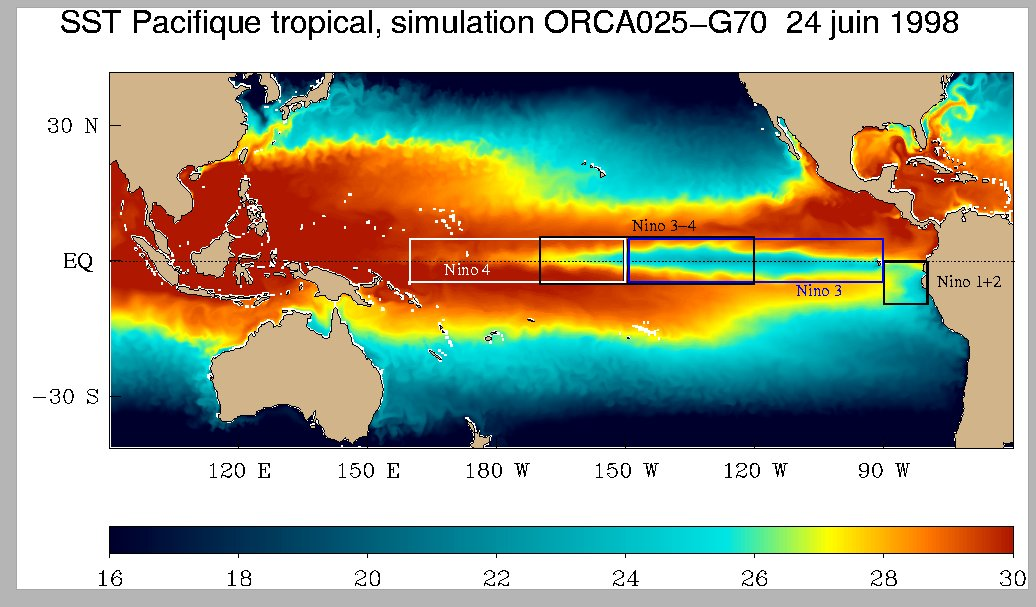
\includegraphics[width=10cm]{FIGURES/ninoboxes.eps}
\caption{Definition of the Nino boxes.}
\end{center}
\end{figure}

\begin{figure}[H]
\begin{center}
%\includegraphics[width=15cm]{FIGURES/ORCA12.L46-MAL95_nino.eps}
\caption{Monthly mean variations of the averaged temperature in el Nino boxes. Model is 
in black and observations (TOA array) are in green. Bottom plot is the Southern Oscillation 
index (monthly fluctuations in the air pressure difference between Tahiti and Darwin: sustained negative values of the SOI often indicate El Nino episodes).}
\end{center}
\end{figure}



% ================================================================
% Acknowledgement
% ================================================================

\section*{Acknowledgement}

This simulation has been performed on Jade supercomputer (CINES) with CPU hours allocated by GENCI (\textcolor{blue}{Grant GENCI X2011XXXXXXX}).



% ================================================================
% Acknowledgement
% ================================================================

\bibliographystyle{plain}
\bibliography{bibliographie}


\end{document}

%---------------------------------------------------------------------------------------------------



